\FloatBarrier
\begin{figure}[h]
\resizebox{\columnwidth}{!}{
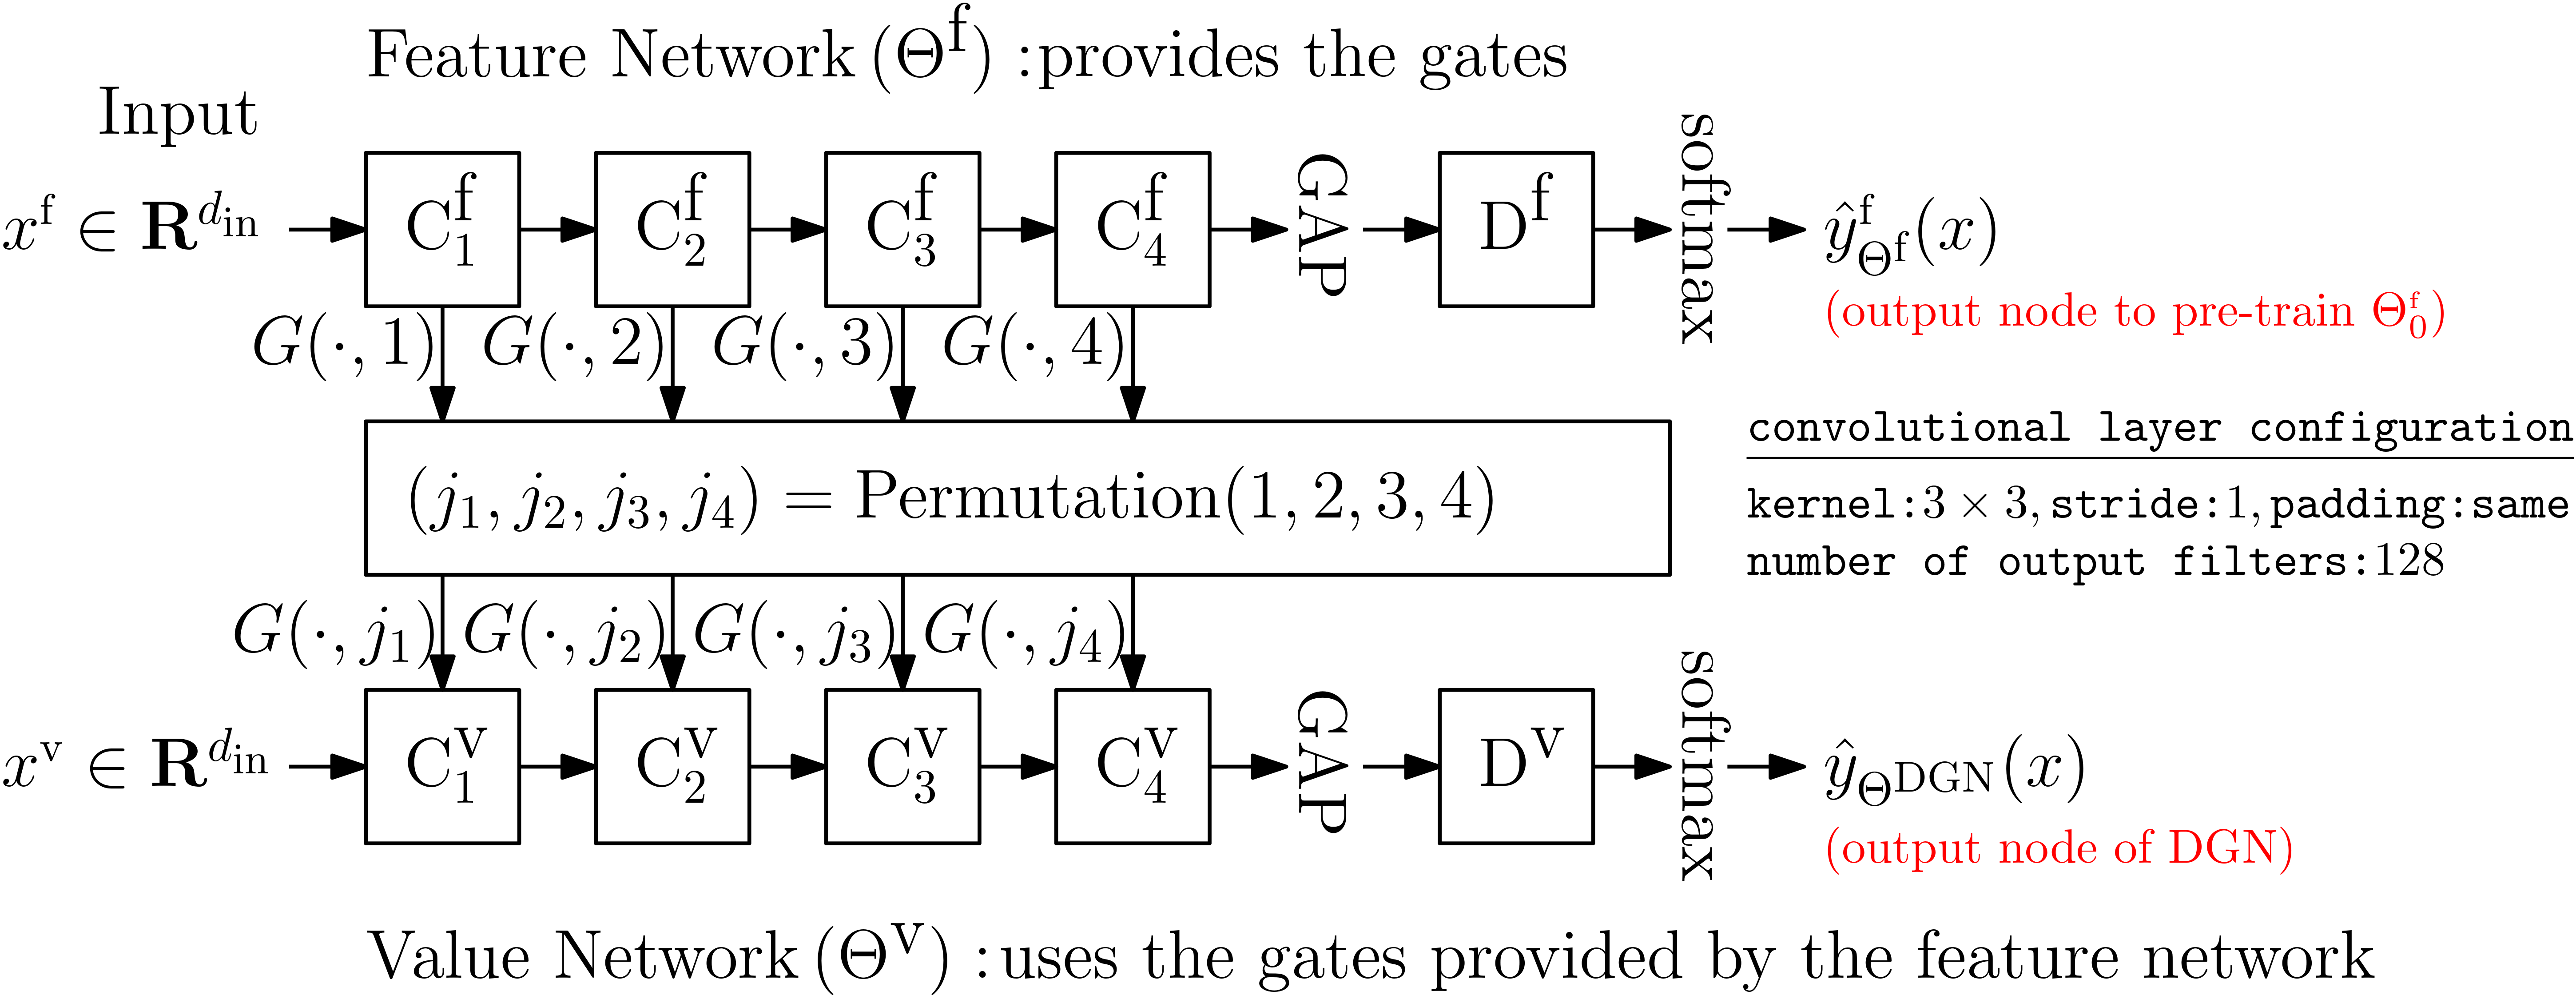
\includegraphics[scale=0.5]{figs/ablation.png}
}
\caption{\small{$\textrm{C}_i^{\text{f}},\textrm{C}_i^{\text{v}},i\in[4]$ are the convolutional layers, which are followed by \emph{global-average-pooling} (GAP) layer then by a dense layer ($\textrm{D}^{\text{f}}$/$\textrm{D}^{\text{v}}$), and a softmax layer to produce the final logits.}} %`R',  `L', `T' and `NT' stand for random, learnt, trainable and non-trainable respectively.}}
\label{fig:ablation}
\end{figure}
\FloatBarrier
\begin{table}[h]
\centering
\begin{tabular}{|p{1cm}|p{1.6cm}|p{1.7cm}p{0.001cm}|}\hline
&\centering{FC (MNIST)}& \centering{CNN (CIFAR-10)}& \\\hline
FR-II& \centering$94.1\%$ & \centering$67.5\%$& \\\hline
FR-DI& \centering$94.1\%$ & \centering$67.6\%$& \\\hline
DL& \centering$98.1\%$ & \centering$77.6\%$&\\\hline
FL& \centering$98.6\%$ & \centering$79.4\%$&\\\hline
ReLU& \centering$98.5\%$ & \centering$80.4\%$&\\\hline
\end{tabular}
\caption{Shows test accuracies in each of the $4$ different regimes. In all the $4$ regimes (FC as well as CNN) the results averaged over the $48$ different modes. In all cases, standard deviation was less than $0.5\%$.}
\end{table}
